\subsection{Quarkonia and Open Heavy Flavor}
\label{Sec:HF}
 Hadrons containing heavy quarks (charm and bottom) play a special role in hot QCD matter studies.
	The heavy-quark masses, $m_{c,b}\simeq1.5,5$\,GeV, are large compared to the temperatures typically
	realized in the medium produced in heavy-ion collisions. This has important consequences.
	First, the production of heavy quarks is essentially restricted to the initial impact of the
	incoming nuclei. After that, they ``diffuse" through the produced medium, much like Brownian
	particles. The modifications of their momentum spectra relative to the initial spectra can thus
	serve as a rather direct measure of their coupling strength to the hot medium. This is so because 
        their thermal relaxation time is increased compared to that for light particles by a factor of order 
        $m_Q/T\simeq$~5-20, implying that heavy quarks in the QGP (or hadrons in hadronic matter) are 
        not expected to fully thermalize over the course of the fireball lifetime, and thus retain a 
        ``memory" of their interaction history. Moreover, at small and intermediate momenta, the heavy-quark 
        interactions become dominantly elastic and may be amenable to a potential-type prescription. 
        In the vacuum, the potential approach is well established for the description of heavy quarkonia, 
        i.e., bound states of a heavy quark and its anti-quark. The vacuum potential is characterized 
        by a color-Coulomb interaction at short distances and a linearly rising ``string" term at 
        intermediate and large distance associated with confinement. When embedded into a QGP, the 
        properties of heavy quarkonia in the QGP will thus reflect the modifications of the in-medium
        QCD potential. With increasing temperature one expects a subsequent dissolution of the 
        bound states, as the medium-induced screening penetrates to smaller distances. However, this
        simple picture is complicated by inelastic collisions with medium particles, leading to 
        a dynamical dissociation of the bound state. These processes generate in-medium widths and
        need to be accounted for in the description of quarkonium spectral functions at finite
        temperature. In heavy ion collisions, the in-medium properties of quarkonia have to be inferred
        from their production yields and momentum spectra in the final state. A thorough interpretation
        of the data thus requires systematic analyses of the centrality, energy and species dependence
        of quarkonia. This usually requires transport approaches to calculate the time evolution of 
        quarkonium distributions including both dissociation reactions and formation processes
        through recombination of diffusing heavy quarks.   
     	In the following we briefly summarize recent progress in both open and hidden heavy flavor probes of
        hot and dense QCD matter.


\subsubsection{Quarkonia Suppression and Enhancement}
\label{Sec:Quarkonia}


Theoretical studies of heavy quarkonia in QCD matter are carried out both from first 
principles using lattice-discretized QCD computations~\cite{Bazavov:2009us,Kaczmarek:2012ne} 
and within  effective model approaches. The latter aid in interpreting the lattice results and 
form the bridge to phenomenological implementations in heavy-ion collisions.

One of the key quantities computed in lattice QCD is the free energy, $F_{Q\bar Q}(r,T)$, 
of a static $Q\bar Q$ pair at distance $r$ in a medium at temperature $T$. In the vacuum it reduces to the well-known Cornell 
potential between the two quarks, but in the medium an additional entropy term develops, 
$F_{Q\bar Q}= U_{Q\bar Q} - T S_{Q\bar Q}$. Accurate calculations for $F_{Q\bar Q}(r,T)$, which are 
now available for full QCD with realistic light quark masses, show marked deviations from 
its vacuum form, through a progressive ``Debye screening" toward smaller distances 
as temperature increases. When utilizing the free energy as a potential in a Schr\"odinger 
equation~\cite{Digal:2001iu}, the charmonium groundstate, \Jpsi\, dissolves slightly above 
the critical temperature, while the excited states melt at or even below $T_{c}$; only the 
bottomonium groundstate, $\Upsilon$, survives up to 2-3\,$T_c$. On the other hand, if the 
potential is approximated with the internal energy, $U_{Q\bar Q}$, the \Jpsi\ survives to 
significantly higher temperatures, possibly up to 2\,$T_c$. These limiting cases are sometimes 
referred to as weak- and strong-binding scenarios, respectively. It has also become clear 
that a proper inclusion of absorptive processes in the $Q\bar Q$ system, characterizing its 
dissociation by dynamical processes, is essential to arrive at a realistic and quantitative description 
of its in-medium properties. 

Lattice computations also provide detailed information on $Q\bar Q$ correlation functions 
in euclidean space-time (where the ``imaginary-time" coordinate is related to the temperature 
of the system). Extracting the physical (real-time) $Q\bar Q$ spectral function requires an 
inverse integral transform on a limited number of ``data" points. This usually is done using 
maximum likelihood methods~\cite{Asakawa:2000tr,Aarts:2007pk}, sometimes guided by a 
parametric ansatz for the spectral function~\cite{Ding:2012sp}. In the bottomonium sector one 
can additionally utilize nonrelativistic heavy-quark effective theory~\cite{Aarts:2014cda}. 
The heavy-quark transport coefficient has been extracted from the low energy limit of the 
spectral functions in quenched QCD (no dynamical 
quarks)~\cite{Banerjee:2011ra,Ding:2012sp,Kaczmarek:2014jga}, highlighting the close connection 
between quarkonia and open heavy flavor in the QGP (cf.~Section~\ref{Sec:OpenHF}). The 
``reconstructed" charmonium spectral functions from lattice QCD have not yet led to definite
conclusions about the fate of bound states in the QGP. A promising complementary source of 
information are spatial correlation functions~\cite{Karsch:2012na,Bazavov:2014cta}; they are 
related to the 3-momentum dependence of the quarkonium spectral functions, but also encode 
information on modifications of the spectral (energy) strength in medium.   

Fruitful connections to lattice QCD results have been established with potential models, 
either through a Schr\"odinger equation~\cite{Mocsy:2005qW} or a thermodynamic $T$-matrix 
formulation~\cite{Cabrera:2006wh}. Here, the calculated  spectral functions can be 
straightforwardly integrated to obtain the euclidean correlation functions computed on the 
lattice. Both strong- and weak-binding scenarios for the $Q\bar Q$ appear to be compatible 
with the lattice data, once absorptive parts and a proper treatment of the continuum are 
included in the calculations. A better discrimination power arises when analyzing the 
interactions of open heavy flavor with the medium. This has been pursued in the $T$-matrix 
approach~\cite{Riek:2010fk}; only the strong-binding scenario produces sufficient strength 
in the heavy-quark transport coefficient to come close to open heavy-flavor observables in 
heavy-ion collisions (cf.~Section~\ref{Sec:OpenHF}).      
Recent progress in the determination of the in-medium $Q\bar Q$ potential has been made by 
utilizing the spectral functions of the so-called Wilson loop correlator, including absorptive
parts~\cite{Burnier:2014ssa}. Here, the real part of the potential turns out to be close to 
the free energy. Further theoretical work, exploiting the insights derived from both lattice QCD and 
effective models, is needed to clarify these issues and arrive at a consistent picture of 
quarkonia and open heavy flavor in the QGP.

To confront (and eventually extract) the equilibrium properties of quarkonia with (from) 
data in heavy-ion experiments, one typically adopts Boltzmann-type transport approaches to 
model the space-time evolution of quarkonium phase-space distributions, from their initial
production until the fireball freezes out. The quarkonium equilibrium properties 
are functions of 
the binding energy, in-medium heavy-quark masses (defining the continuum threshold) 
and inelastic reaction rates, e.g., $g$ + \Jpsi\ $\rightarrow$ $c$ + $\bar c$. In some 
approaches~\cite{Zhao:2010nk,Emerick:2011xu}, the in-medium quarkonium properties 
implemented into the transport equation have been checked against the euclidean correlators 
from lattice-QCD described above. Here too, current heavy ion phenomenology appears to favor a
strong-binding scenario~\cite{Zhao:2010nk,Liu:2010ej,Emerick:2011xu,Strickland:2011aa},
which would be consistent with the phenomenology for open heavy flavor.

The principle of detailed balance requires that one account for quarkonium formation reactions 
(called ``regeneration" or ``coalescence"), if the quarkonium state under 
consideration exists at the local medium temperature (relative to the ``melting temperature"). 
An accurate assessment of quarkonium formation reactions not only requires knowledge of the 
reaction rate, but also of the phase-space distributions of open heavy flavor. Again, this 
couples the problem of quarkonium production with heavy-flavor diffusion,
providing both challenges and opportunities. 

The quarkonium transport equations need to be evolved over a realistic space-time 
evolution of a given collision system and energy. Current approaches include expanding 
thermal fireball models with QGP and hadronic phase~\cite{Grandchamp:2003uw,Zhao:2010nk} 
or co-mover interactions~\cite{Capella:2007jv}, ideal hydrodynamics~\cite{Zhu:2004nw}, and
viscous hydrodynamics with local momentum anisoptropies~\cite{Strickland:2011aa}. Systematic investigations
of how sensitive the final results are to details of medium evolution models need to be 
conducted. Most of the calculations include cold nuclear matter (CNM) effects to construct 
the initial conditions of the quarkonium phase space distributions, as well as a gain 
term in the rate equation which is essential for a realistic description of charmonia 
at collider energies. For the $\Upsilon$ states, regeneration effects seem to be rather 
small, even at the LHC~\cite{Emerick:2011xu}.
Quarkonium production has also been evaluated via statistical recombination at the
QCD phase boundary~\cite{BraunMunzinger:2000px,Andronic:2003zv,Andronic:2007bi}. In essence,
this approach corresponds to the equilibrium limit of the transport approaches, but it 
allows for a more complete incorporation of open and hidden charm hadrons to account for 
their relative chemical equilibrium (at fixed charm-quark number).



	
An extensive program of \Jpsi\ measurements in A+A collisions has been carried out at the SPS
($\sqrt{s_{NN}}$ = 17.3 GeV), RHIC ($\sqrt{s_{NN}}$ = 200 GeV) and the LHC ($\sqrt{s_{NN}}$ = 2.76 TeV).
These measurements were motivated by the possibility of observing signals of color deconfinement through the
suppression of \Jpsi\ in the case of QGP formation\cite{Matsui:1986dk}. In fact, a strong suppression of the \Jpsi\ is observed
at all three energies, but it has become clear that the manifestation of color screening in the observed
modifications can not be uniquely determined without a good understanding of two significant competing effects.
The first of these is the modification of \Jpsi\ production cross sections in a nuclear target (known as
cold nuclear matter effects); it has been addressed at RHIC using d+Au collisions and at the SPS and LHC
using p+Pb collisions. The second effect is the recombination of charm and anticharm discussed above.

	
Using p+Pb and d+Au data as a baseline, and under the assumption that cold nuclear matter effects
can be factorized from hot matter effects, the suppression in central collisions due to the presence of
hot matter in the final state has been estimated to be about 25\% for Pb+Pb at the SPS~\cite{Arnaldi:2010ky},
and about 50\% for Au+Au at RHIC~\cite{Brambilla:2010cs}, both measured at midrapidity. The modification
of \Jpsi\ production in Au+Au collisions has been measured at $\sqrt{s_{NN}}$=39, 62 and 200 GeV 
by PHENIX~\cite{Adare:2012wf}
and STAR~\cite{Adamczyk:2013tvk,Zha:2014nia}.
The results for the rapidity range $1.2 < |y| < 2.2 $ is shown in Figure~\ref{fig:PHENIX_excitation_function}, 
where it is compared with a theoretical
calculation~\cite{Zhao:2010nk} that includes cold nuclear matter effects and the effects of regeneration.
The experimental observation is that the modification is similar at all three collision energies, in spite of the
differences in energy density.
Similar observations apply to data measured by STAR at mid-rapidity ($|y| < 1$)~\cite{Adamczyk:2013tvk,Zha:2014nia}.
In the model calculation, this is expected because the increased direct suppression at the 
higher energy due to stronger Debye screening is nearly compensated by the increase in the regeneration 
component~\cite{Grandchamp:2001pf}.
	
\begin{figure}[!htb]
\centerline{
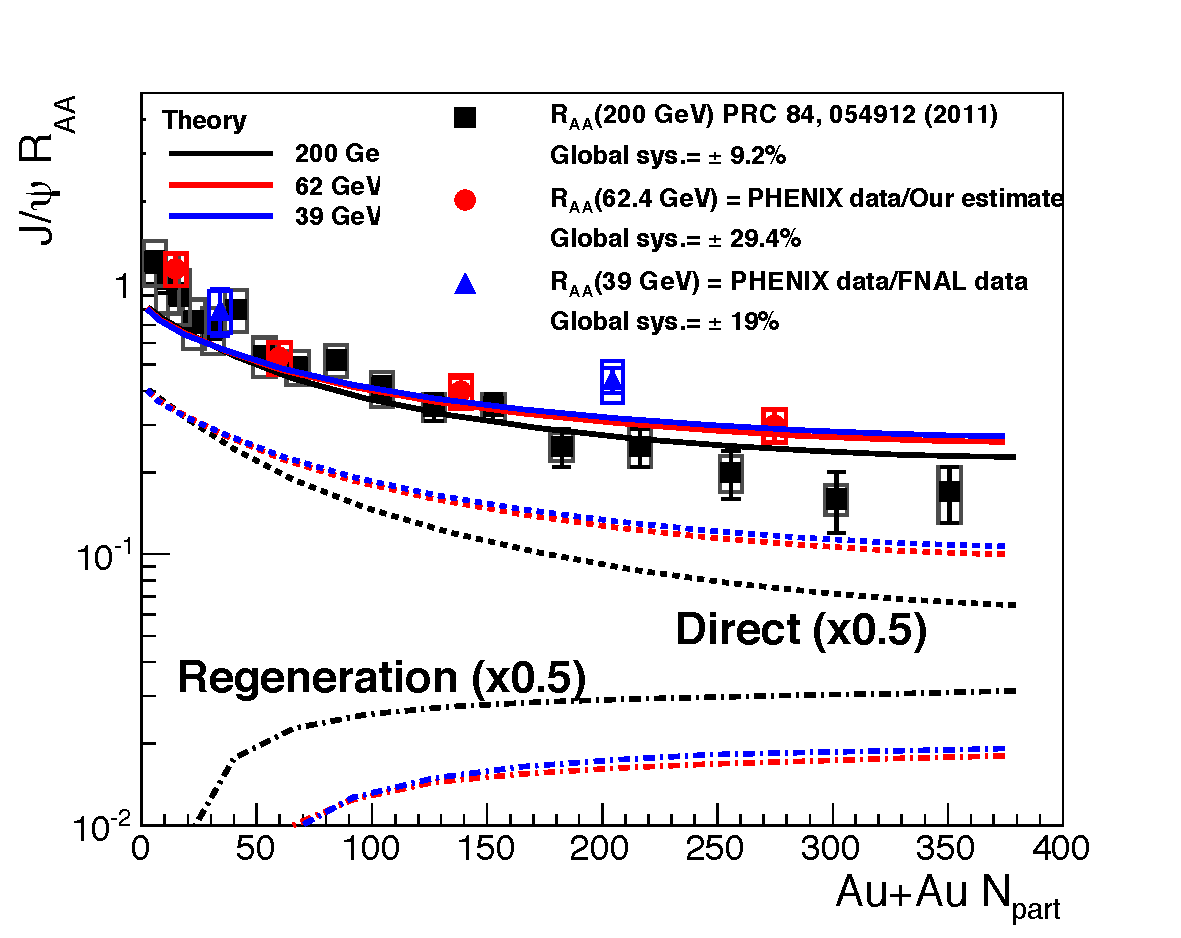
\includegraphics[width=0.8\textwidth]{fig/PHENIX_AuAu_excitation_function}
}
\caption[PHENIX data for \Jpsi\ production compared to theory calculations]{The nuclear modification factor for \Jpsi\ production for $\sqrt{s_{NN}}$=200, 62 and 39~GeV \AuAu\ collisions from
PHENIX~\cite{Adare:2012wf}, compared with theory calculations~\cite{Zhao:2010nk} showing the contributions from direct
suppression and regeneration.
}
\label{fig:PHENIX_excitation_function}
\end{figure}
%\begin{figure}[!ht]
%\centerline{
%\includegraphics[width=0.480\textwidth]{fig/ALICE_PHENIX_RAA_vs_dnchdeta}
%\includegraphics[width=0.48\textwidth, height=0.458\textwidth]{fig/PHENIX_ALICE_Jpsi_pT_comparison}
%}
%\caption{Left: Comparison of the nuclear modification factor for $J\psi$ production for $\sqrt{s_{NN}}=200$~GeV \AuAu\ collisions from
%PHENIX and for $\sqrt{s_{NN}}=2.76$~TeV \PbPb\ from ALICE. The data are plotted versus the charged
%particle multiplicity at midrapidity, which is used as a rough proxy for energy density. Right: The transverse momentum
%distributions for the same data sets, showing the low momentum enhancement that would be expected from a
%large coalescence contribution at the LHC energy.
%}
%\label{fig:ALICE_PHENIX_Jpsi_RAA}
%\end{figure}

\begin{figure}[!ht]
 \centering
 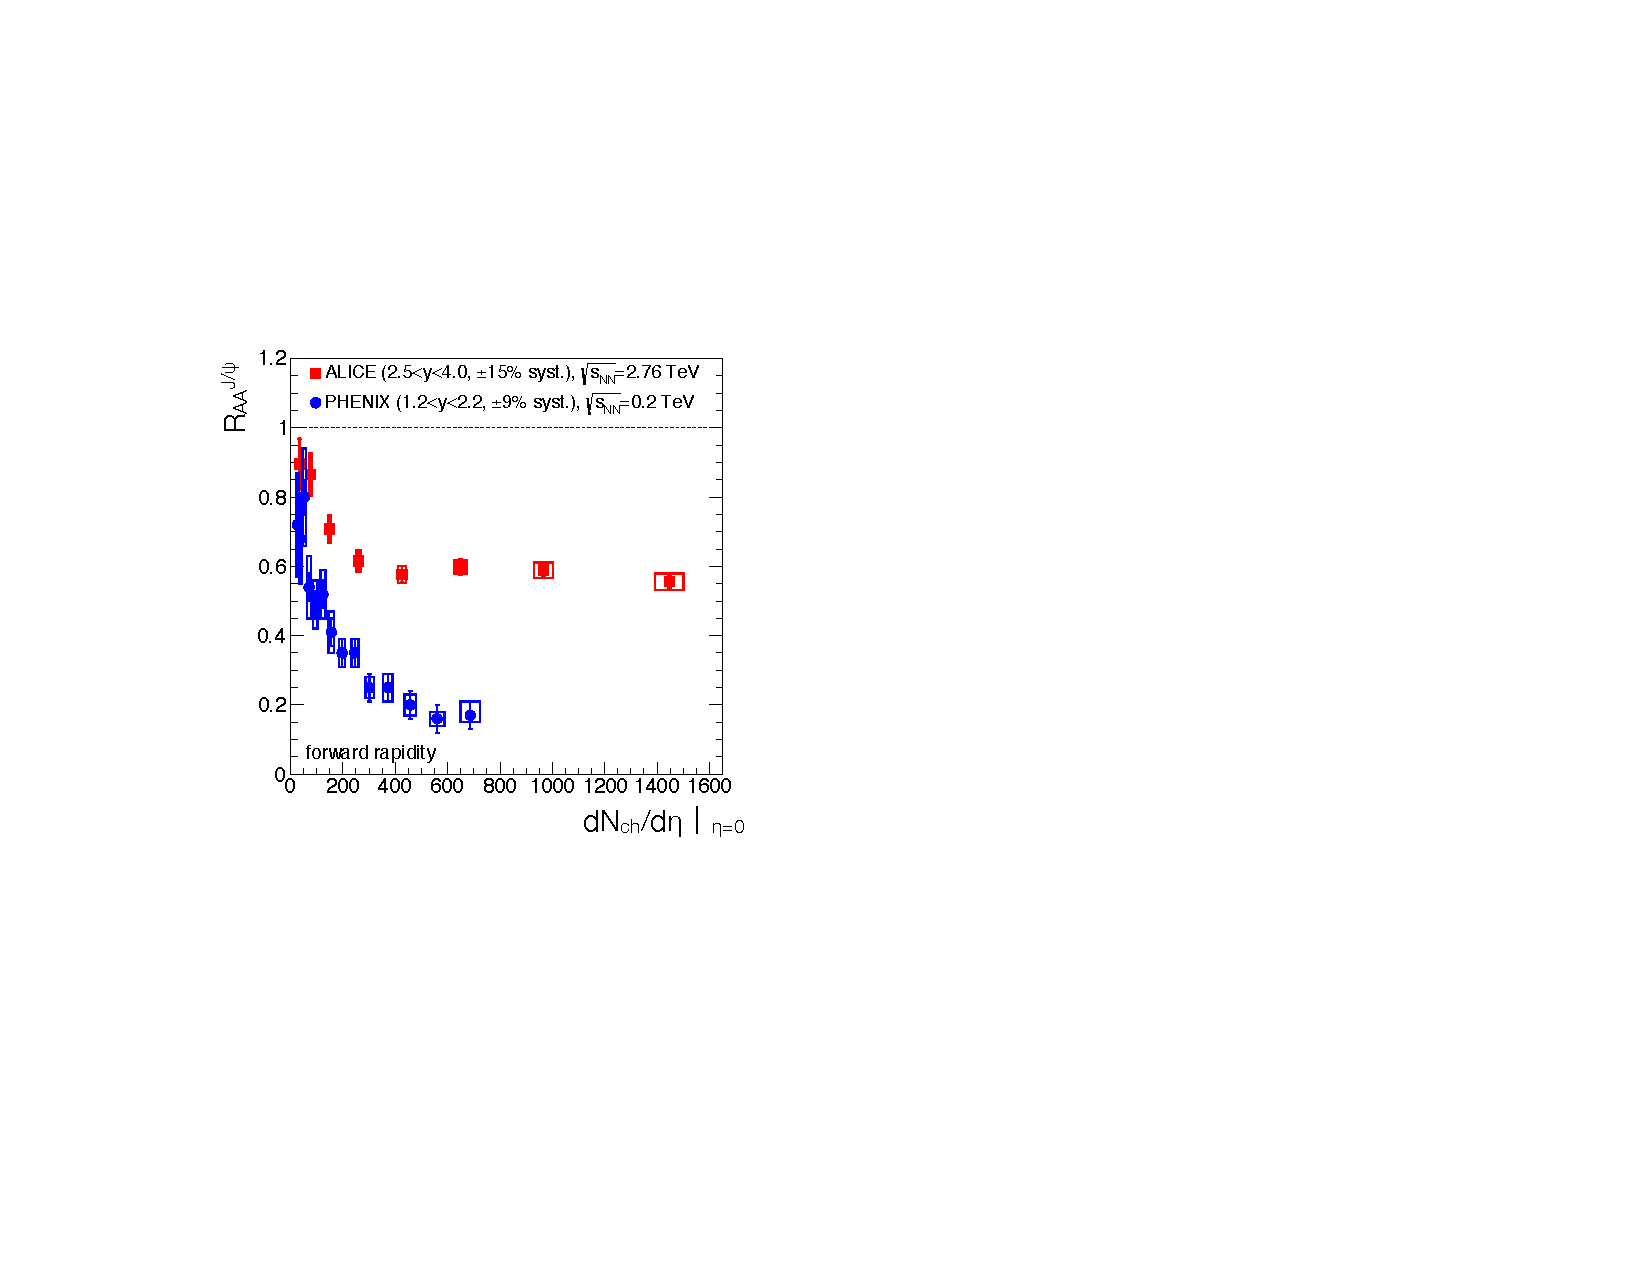
\includegraphics[width=0.435\linewidth]{fig/ALICE_PHENIX_Jpsi_cropped}
 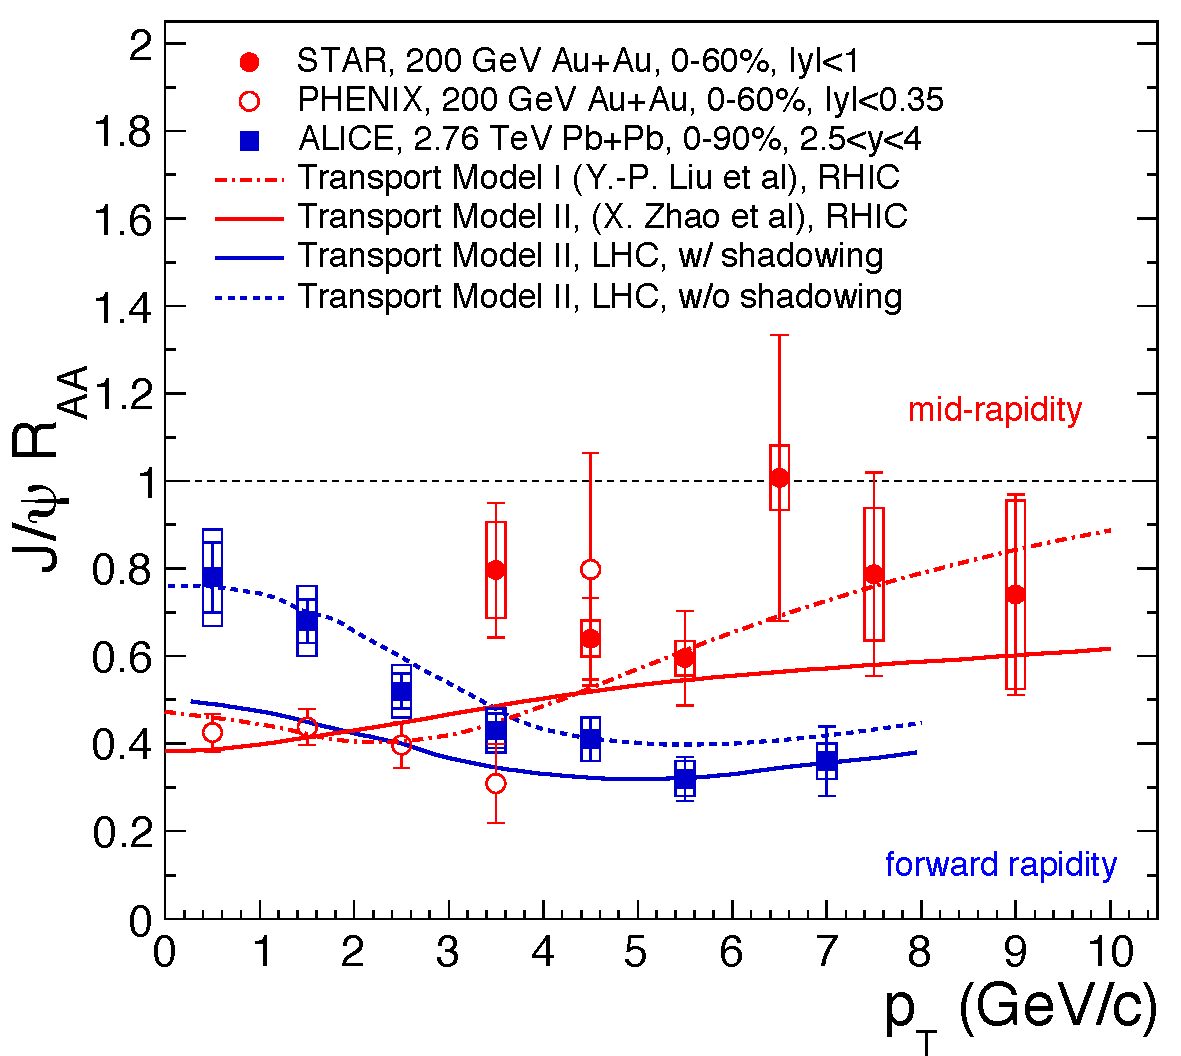
\includegraphics[width=0.46\linewidth]{fig/Jpsi_raa_vs_pt}
 \caption[Comparison of RHIC and LHC data on \Jpsi\ production]{
 Left: Comparison of the nuclear modification factor for \JPsi\ production for $\sqrt{s_{NN}}=200$~GeV \AuAu\ collisions from
PHENIX and for $\sqrt{s_{NN}}=2.76$~TeV \PbPb\ from ALICE~\cite{Andronic:2014zha}. The data are plotted versus the charged
particle multiplicity at midrapidity, which is used as a rough proxy for energy density. 
Right: The transverse momentum
distributions for the same data sets,
together with higher-momentum data from STAR\cite{Adamczyk:2012ey}
showing the low momentum enhancement that would be expected from a
large coalescence contribution at the LHC energy.
The data are compared to a transport model\cite{Liu:2009nb}
which incorporates the effects of gluon scattering and coalescence.
}
\label{fig:ALICE_PHENIX_Jpsi_RAA}
\end{figure}
	
	
The first \Jpsi\
data in Pb+Pb collisions at $\sqrt{s_{NN}}$ = 2.76 TeV from ALICE~\cite{Abelev:2012rv}, measured at forward
rapidity, are shown alongside forward rapidity PHENIX data in the left panel of Figure~\ref{fig:ALICE_PHENIX_Jpsi_RAA}. 
The suppression in central collisions is found to be far greater at RHIC than at the LHC. A similar result is found
at midrapidity. This is consistent with a predicted~\cite{Zhao:2011cv} strong coalescence component due to the 
large production rate of charm and anti-charm quarks in a central collision at the LHC. This explanation is 
corroborated by the transverse-momentum spectra~\cite{Adare:2006ns,Adamczyk:2012ey,Abelev:2013ila}, 
which exhibit the expected~\cite{Zhao:2011cv,Liu:2009nb}
low-momentum enhancement generated by the coalescence contribution, 
as shown in the right panel of 
Figure~\ref{fig:ALICE_PHENIX_Jpsi_RAA}.


\begin{figure}[!htb]
\centerline{
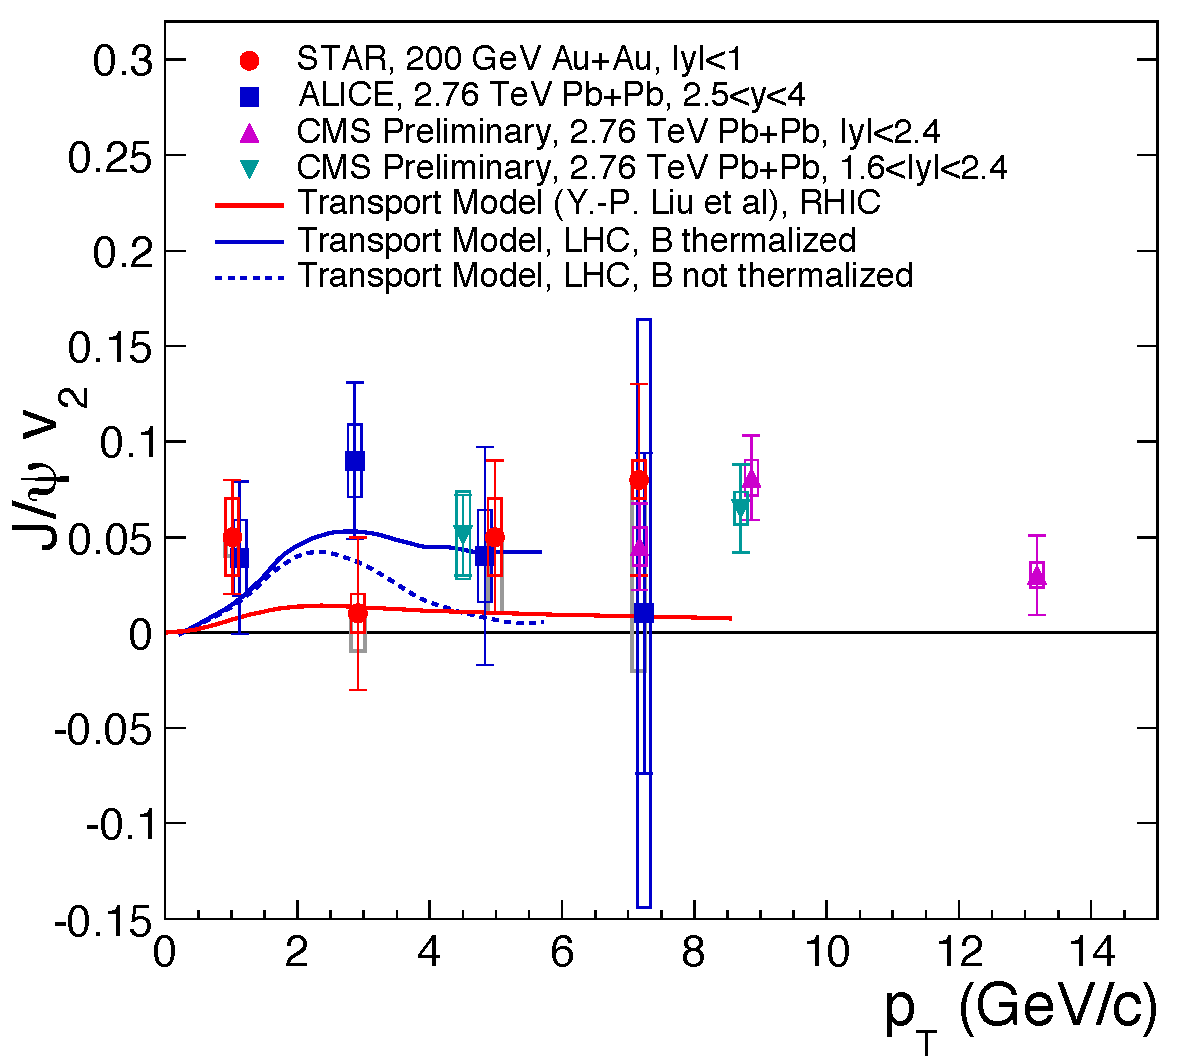
\includegraphics[width=0.8\textwidth]{fig/Jpsi_v2}
}
\caption[\Jpsi\ elliptic flow measurements at RHIC and LHC compared to theory]{
The transverse momentum dependent elliptic flow measurements of
\Jpsi\'s from STAR\cite{Adamczyk:2012pw}, ALICE\cite{ALICE:2013xna}, and CMS\cite{Moon:2014lia} compared with the theoretical calculations\cite{Liu:2009gx}.
}
\label{Fig:JPsi_v2}
\end{figure}

One of the crucial tests of the combined effects of color screening
and coalescence in \Jpsi\ production is provided by the measurement of the \Jpsi\ elliptic flow.
All other hadrons acquire flow velocities through their interaction with 
the QGP medium and simultaneously exhibit
significant elliptic flow and strong nuclear suppresssion. 
In contrast, disassociation of \Jpsi\'s from color screening
is predicted to result in strong nuclear modification with the absence of a flow signal, while
\Jpsi\'s later regenerated from coalescence production will carry flow from the thermalized charm quarks from which they are formed. 
Figure~\ref{Fig:JPsi_v2} 
shows the transverse momentum dependent elliptic flow measurements\cite{Adamczyk:2012pw,ALICE:2013xna,Moon:2014lia} 
from RHIC and the LHC together with a corresponding theoretical calculation\cite{Liu:2009gx}.
The data are consistent (within the current large statistical errors) with a model incorporating
disassociation from color screening at both RHIC and the LHC in combination with
significant regeneration of \Jpsi\'s at the LHC from coalescence of thermalized charm and anti-charm quarks,
The larger role of the coalescence  mechanism at the LHC results from the much 
higher cross section for charm production in the initial phase of the collision at LHC energies as compared to RHIC.
There is great promise that the  future availability of data sets 
with improved statistical precision
at the widely spaced collision energies of RHIC and the LHC, 
in combination with studies constraining CNM effects with \pA\ data, 
will lead to a quantitative
understanding of the role of coalescence from nearly thermalized charm and anti-charm quarks.
However, a more direct window on the Debye screening and dissociation effects alone is expected from
a systematic analysis of bottomonium production, as we will now discuss.
		
Bottomonium production is believed to have several advantages over charmonia as a probe of deconfinement in the
QGP. First, the $\Upsilon(1S)$, $\Upsilon(2S)$ and $\Upsilon(3S)$ states can all be observed with comparable
yields via their dilepton decays. Second, bottom production in central collisions is $\sim$ 0.05 pairs at RHIC
and $\sim$ 5 pairs at LHC~\cite{Brambilla:2010cs}. At RHIC, one expects this to effectively remove any contributions
from coalescence of bottom and anti-bottom quarks (although some care has to be taken, since the ratio of bottomonium over
open bottom states in pp collisions is $\sim$0.1\% and thus a factor of 10 smaller than in the charm
sector; thus, even small regeneration, even from a single pair in the reaction, can potentially be significant).
This makes the $\Upsilon$ suppression at RHIC dependent primarily on color screening and dissociation reactions,
as well as cold nuclear matter effects. Recent theoretical calculations~\cite{Emerick:2011xu} support the
assertion that the coalescence production for $\Upsilon$'s is small at RHIC. At LHC energies, 
bottom coalescence could become comparable with charm coalesence at RHIC, i.e. at the 10's of percent level.
Since the $\Upsilon(1S)$, $\Upsilon(2S)$ and $\Upsilon(3S)$ have a broad range of radii, precise measurements
of bottomonia modifications at RHIC and LHC energies will provide information over a large range of
binding energies at two widely different initial temperatures, for a case where the modification is dominated
by Debye screening effects.
	
The CMS experiment at the LHC has mass resolution that is sufficient to cleanly separate all three of the
$\Upsilon$ states at midrapidity using dimuon decays~\cite{Chatrchyan:2012lxa}. The data obtained in Pb+Pb collisions at
$\sqrt{s_{NN}}$=2.76 TeV for the $\Upsilon(1S)$ and $\Upsilon(2S)$ states are shown in
Figure~\ref{fig:CMS_Upsilons}, where they are compared with a model calculation~\cite{Emerick:2011xu} that includes
both cold nuclear matter effects and regeneration. The data show much stronger suppression of the $\Upsilon(2S)$
than the $\Upsilon(1S)$. The $\Upsilon(3S)$ is even more strongly suppressed, 
and as a result the yield is too small to determine accurately the nuclear suppression factor. 
The theory is in good agreement with the data, although better statistical precision is needed for strong
theoretical constraints. Future Pb+Pb data at the LHC will be measured at $\sqrt{s_{NN}}$=5.5 TeV, and will have greatly increased
statistical precision.
	
	
\begin{figure}[!htb]
\centerline{
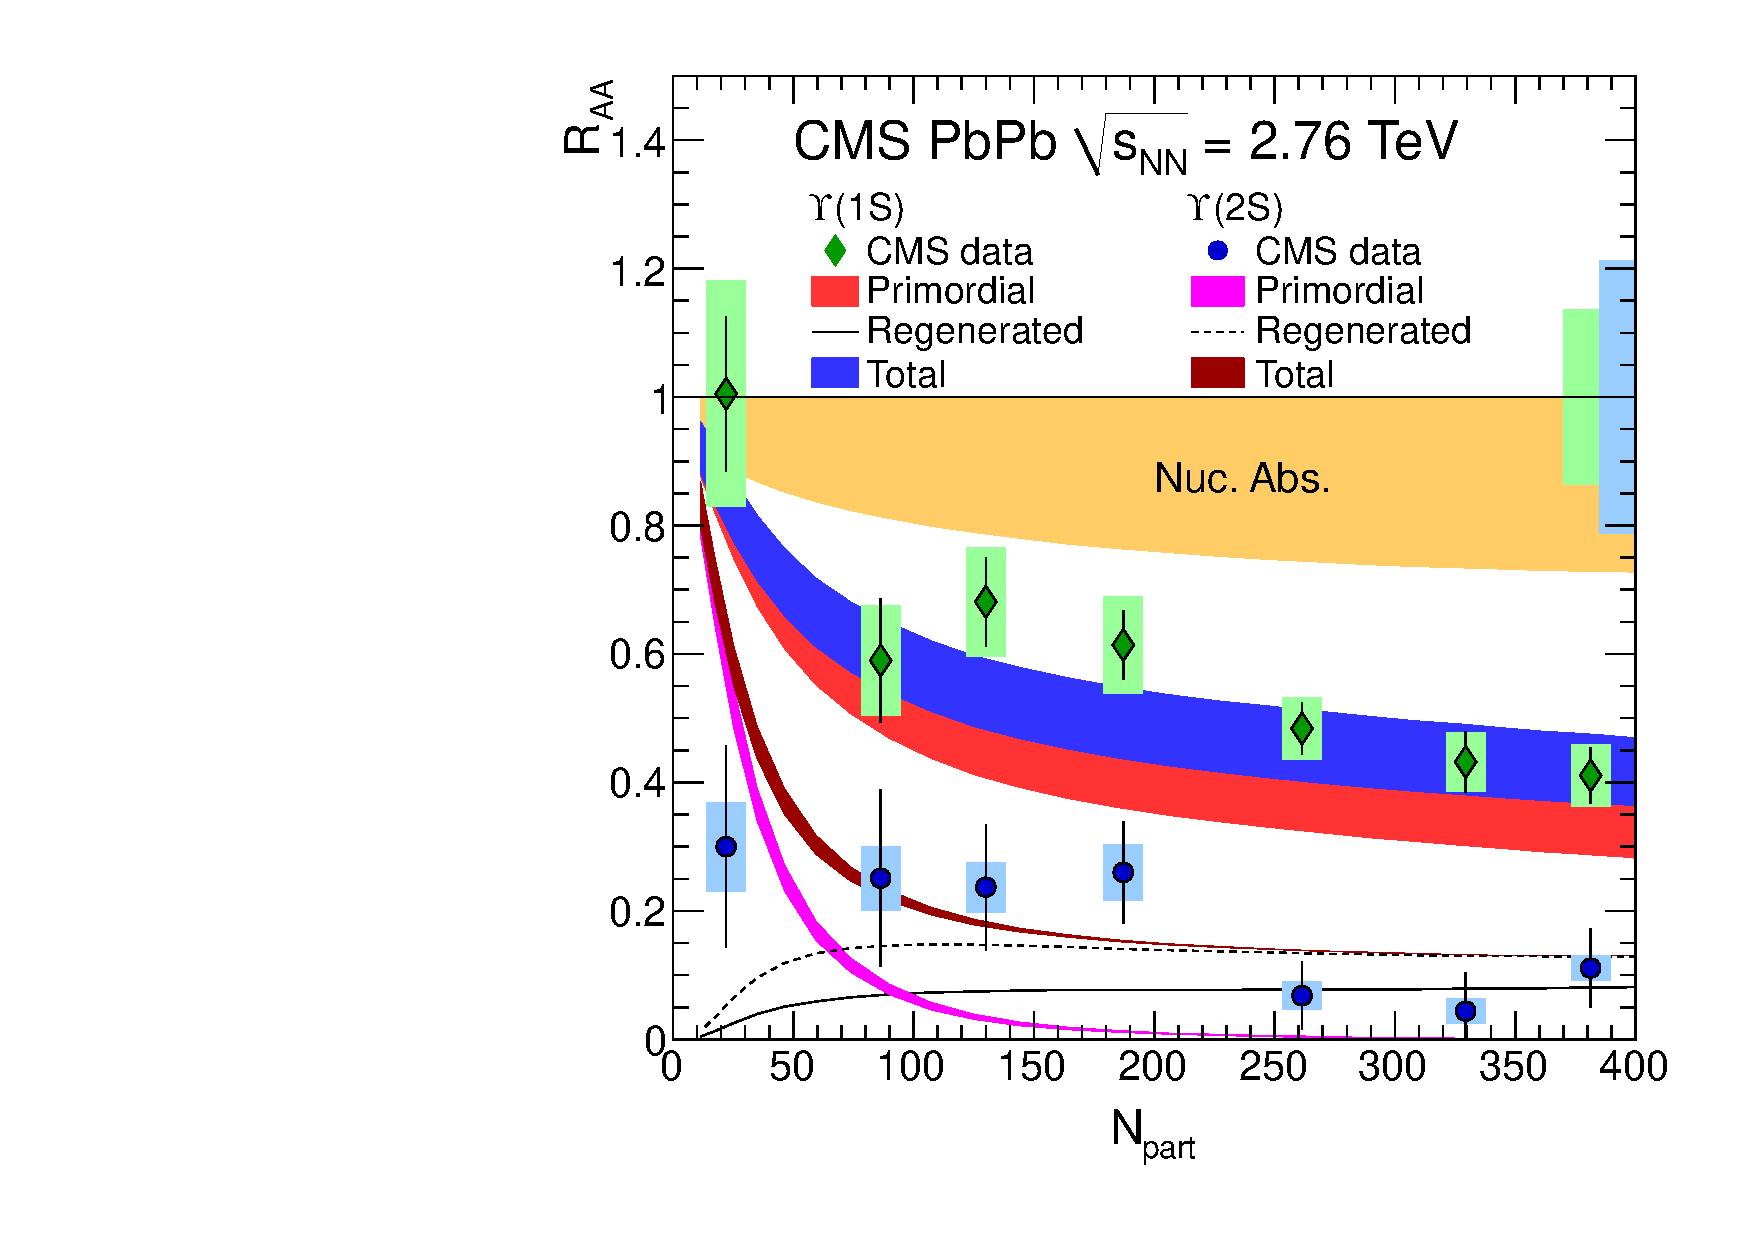
\includegraphics[width=0.7\textwidth]{fig/CMS_Upsilon_RAA_Rapp_theory}
}
\caption[CMS measurements of $\Upsilon$ production compared to theory]{The nuclear suppression factor $R_{AA}$ for the $\Upsilon(1S)$ and $\Upsilon(2S)$ states measured at $\sqrt{s_{NN}}$=2.76 TeV
by CMS~\cite{Chatrchyan:2012lxa}. The theory calculation~\cite{Emerick:2011xu} includes cold nuclear matter effects
and the contributions from the surviving primordial \Jpsi\ and those which are formed by regeneration are shown, as well
as the total.
}
\label{fig:CMS_Upsilons}
\end{figure}
	
	
By the end of Run 3 at
the LHC (approximately 2023) CMS will have measured very precise cross sections for the three
$\Upsilon$ states in p+p, p+Pb and Pb+Pb collisions. A mass-resolved measurement of the modifications
of the three upsilon states with similar precision at RHIC energy would be extremely valuable for all of
the reasons outlined above. However $\Upsilon$ measurements at RHIC have been hampered by a
combination of low cross sections and acceptance, and insufficient momentum resolution to resolve the
three states. At RHIC there are measurements of the modification of the three states
combined in Au+Au by PHENIX~\cite{Adare:2014hje} and STAR~\cite{Adamczyk:2013poh}. These data
are shown in Figure~\ref{fig:RHIC_Upsilons}, along with two theory
calculations\cite{Emerick:2011xu,Strickland:2011aa} of the modification of the three Upsilon states combined.
The data available so far have limited statistical precision, and do not place strong constraints on models.
	
\begin{figure}[!htb]
\centerline{
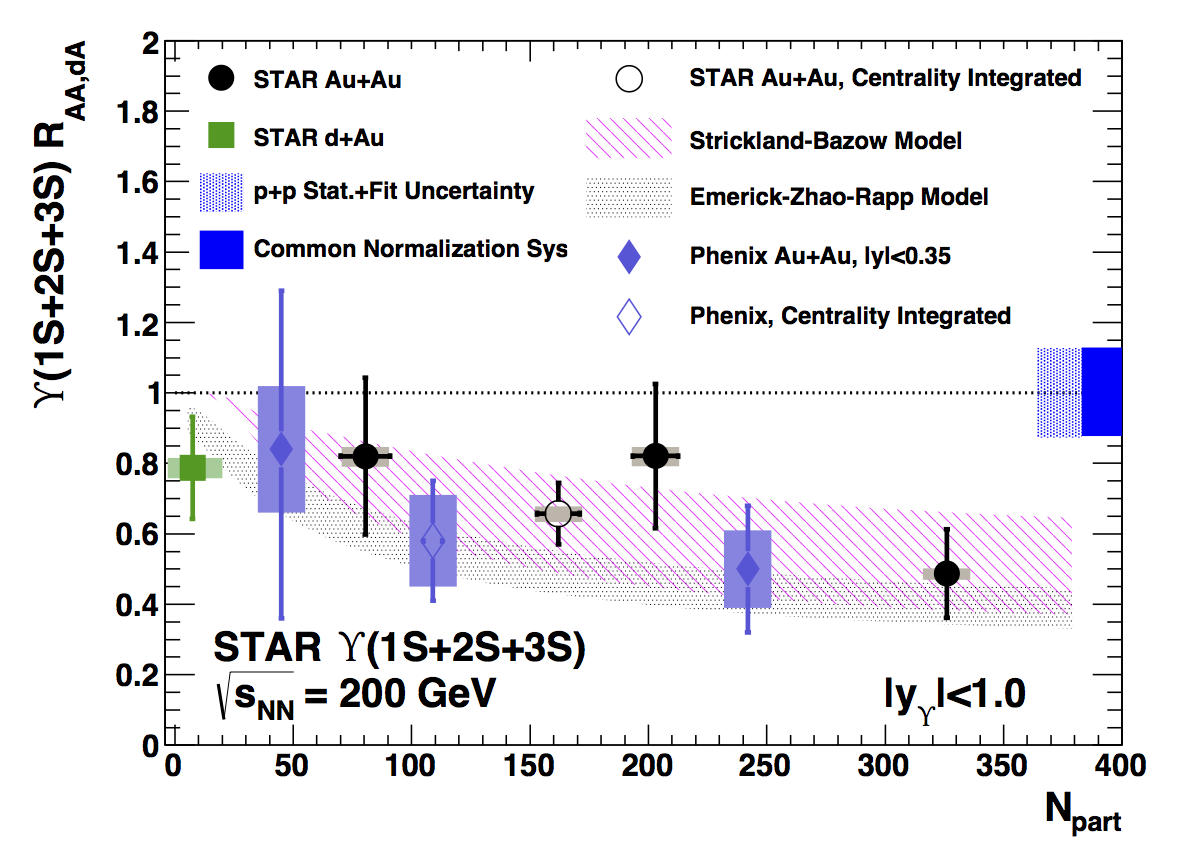
\includegraphics[width=0.9\textwidth]{fig/RHIC_Upsilons}
}
\caption[RHIC measurements of $\Upsilon$ production compared to theory]{The nuclear suppression factor $R_{AA}$ for the $\Upsilon(1S+2S+3S)$ states measured at $\sqrt{s_{NN}}$=200 GeV
by PHENIX\cite{Adare:2014hje} and STAR~\cite{Adamczyk:2013poh}. The theory calculations are from~\cite{Emerick:2011xu,Strickland:2011aa},
}
\label{fig:RHIC_Upsilons}
\end{figure}
	
There are, however, good prospects for future $\Upsilon$ measurements at RHIC. STAR recorded data in the 2014
RHIC run with the new Muon Telescope Detector (MTD), which measures dimuons at midrapidity~\cite{Ruan:2009ug}.
The MTD has coverage of $|\eta| < 0.5$, with about 45\% effective azimuthal coverage. It will have a
muon to pion enhancement factor of $\sim$ 50, and the mass resolution will provide a clean separation
of the $\Upsilon(1S)$ from the $\Upsilon(2S+3S)$, and likely the ability to separate the 2S and 3S states by fitting.
	
On a longer time scale, the proposed sPHENIX detector~\cite{Aidala:2012nz} at RHIC 
discussed in Section~\ref{Sec:FacilitiesFuture} would begin operation in
2021. It is designed to measure $\Upsilon$'s via their dielectron decays at midrapidity. The 100 MeV mass
resolution is sufficient to cleanly separate all three $\Upsilon$ states. Pions are suppressed relative to electrons
by a factor of 90. A combination of very high luminosity, good mass resolution, good background rejection and large
acceptance (about a factor of 7 larger than the MTD) leads to a data set with precision comparable to that expected
from the CMS data by 2023, and on a similar time scale.

%%%%%%%%%%%%%%%%%%%%%%%%%%%%%%%%%%%%%%%%%%%%%
\subsubsection{Open Heavy Flavor Dynamics}
	\label{Sec:OpenHF}
%%%%%%%%%%%%%%%%%%%%%%%%%%%%%%%%%%%%%%%%%%%%%

 The diffusion of a heavy particle through a heat bath of light particles can be 
 quantified by the spatial diffusion coefficient $D_s$. In 
 relativistic systems, such as the QGP, it is convenient to express this transport 
 coefficient in units of the thermal wavelength of the medium, $1/2\pi T$. This renders 
 $D_s(2\pi T)$ a dimensionless quantity which characterizes the (inverse) coupling 
 strength of the diffusing particle to the medium. As such, it is expected to be 
 proportional to the ratio of shear viscosity to entropy, $\eta/s$. For example, in 
 the strong coupling limit of conformal field theories, one has 
 $D_s(2\pi T) \simeq 1$~\cite{Herzog:2006gh,CasalderreySolana:2006rq} and 
 $\eta/s=1/4\pi$ (where small values for each of these quantities indicate strong coupling). 
 
In contrast to the result for strongly coupled theories, perturbative systems
generate much large values for the heavy quark diffusion coefficient. For example,
early calculations based on perturbative methods of the diffusion coefficient for charm and bottom quarks in 
 a QGP~\cite{Svetitsky:1987gq} produced values 
 of $D_s(2\pi T) \simeq 30 \sim {\cal O}(1/\alpha_s^2)$ for a strong coupling 
 constant of $\alpha_s\simeq$~0.3-0.4,  and with a value varying only weakly with temperature. 
 We now know from a 
 phenomenological point of view that these values for $D_s$ are too large to account for 
 the open heavy-flavor (HF) observables in heavy-ion collisions at RHIC and 
 the LHC~\cite{Rapp:2009my}. Later it was found that the formal convergence of the 
 perturbative series requires much smaller values for $\alpha_s$~\cite{CaronHuot:2008uh}. 
 This calls for nonperturbative methods to assess the heavy-flavor diffusion 
 coefficient in QCD matter.  
 
 \begin{figure}[tbh]
 \centerline{ 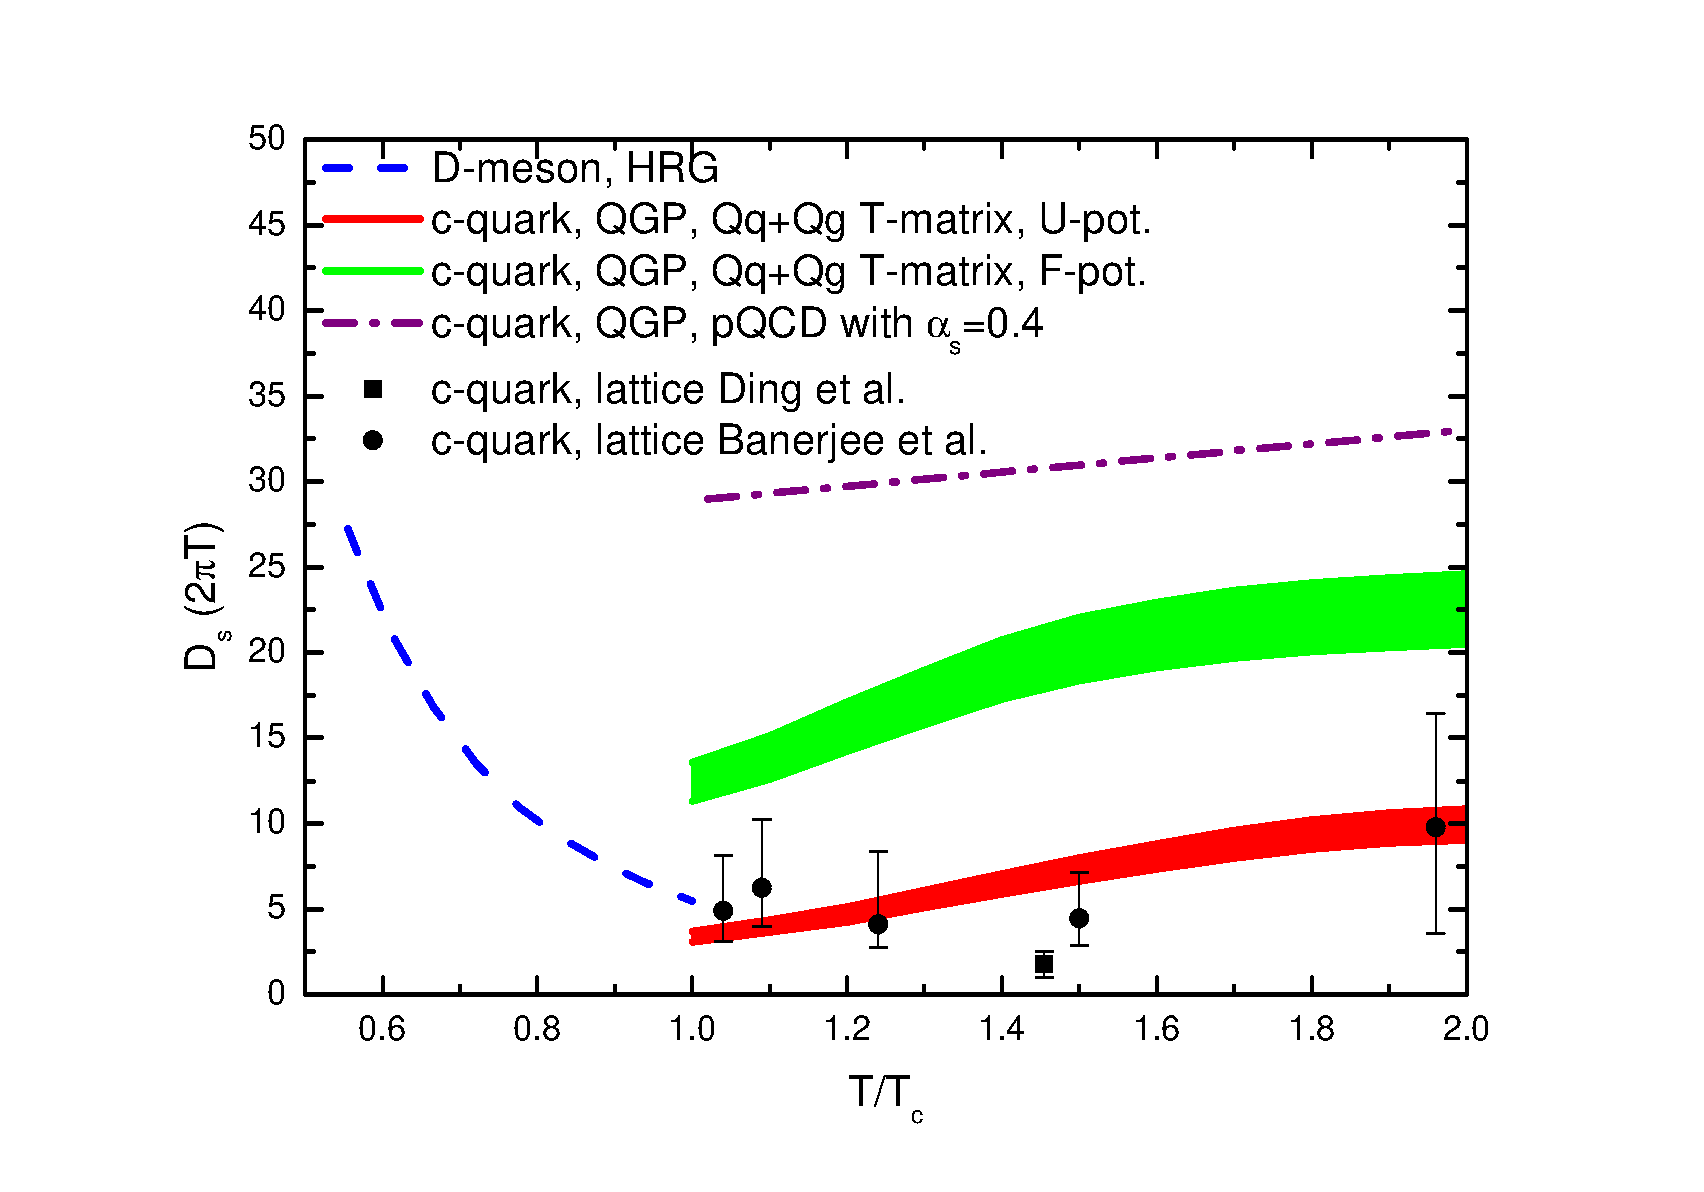
\includegraphics[width=1.00\textwidth]{fig/Ds-2piT} }
 \caption[Spatial diffusion coefficient for charm quarks and $D$-mesons]{Spatial diffusion coefficient for charm quarks in the QGP ($T>T_{\rm c}$)
 and $D$-mesons in hadronic matter ($T<T_{\rm c}$), in units of the thermal wavelength.
 The data points are extracted from quenched 
 lattice QCD~\cite{Banerjee:2011ra,Ding:2012sp,Kaczmarek:2014jga} while the bands are 
 obtained from potential-based $T$-matrix calculations~\cite{Riek:2010fk,Huggins:2012dj} 
 using either the free (green) or internal (red) energies from lattice QCD. The dash-dotted 
 line corresponds to leading order perturbation theory~\cite{Svetitsky:1987gq}.
 }
 \label{fig:Ds-2piT}
 \end{figure}
 Progress has been made to extract $D_s$ from first principles in thermal lattice QCD, 
 by computing euclidean heavy-quark (HQ) correlation functions and reconstructing the 
 low-energy limit of the pertinent spectral function (which defines the transport coefficient). 
 Thus far this has been done in quenched QCD (i.e., in a gluon plasma without dynamical 
 quarks)~\cite{Banerjee:2011ra,Ding:2012sp,Kaczmarek:2014jga}, resulting in a range of 
 values of $D_s(2\pi T) \simeq$~2-6 for temperatures between 1-2~$T_c$, as shown in 
 Figure~\ref{fig:Ds-2piT}. 
 To make closer contact to experiment, it will be necessary to extend these studies 
 to QCD with dynamical quarks, and to compute the 3-momentum dependence of the transport 
 coefficient. The latter can be alternatively expressed through the thermal relaxation 
 rate, $\gamma_Q=T/(m_Q D_s)$, where $m_Q$ is the HQ mass in the QGP, or heavy-meson mass 
 in hadronic matter. 
 
 Non-perturbative calculations of the HQ transport coefficients have also been carried out 
 in the thermodynamic $T$-matrix formalism~\cite{vanHees:2007me,Riek:2010fk,Huggins:2012dj}, 
 which is based on a potential approximation for HQ scattering off thermal partons. The 
 in-medium potential can, in principle, be extracted from thermal lattice QCD, see, e.g., 
 Ref.~\cite{Burnier:2014ssa}. Current uncertainties are usually bracketed by employing 
 either the HQ internal or free energies from the lattice. Using the internal energy one 
 finds values of $D_s(2\pi T)\simeq$\,3-5 at temperatures close to $T_{\rm c}$, increasing 
 to about 10 at 2\,$T_{\rm c}$, for both charm and bottom quarks, see Figure~\ref{fig:Ds-2piT}. 
 For the free energy, the $D_s$ values are about a factor of 2-4 larger. The relaxation 
 rates from the $T$-matrix formalism predict an appreciable 3-momentum dependence, decreasing 
 toward perturbative values at high momenta. Close to $T_{\rm c}$, resonant structures develop 
 in the heavy-light quark $T$-matrices, suggestive of the onset of hadronization. 
 
 Recent work has demonstrated the importance of also treating the  $D$ meson diffusion in the hadronic 
 phase. The pertinent transport coefficient has been estimated 
 in heavy-meson chiral perturbation theory~\cite{Laine:2011is} and in effective 
 hadronic theories including resonance 
 scattering~\cite{He:2011yi,Ghosh:2011bw,Abreu:2011ic,Tolos:2013kva}. The $D$-meson 
 diffusion coefficient significantly decreases as $T_{\rm c}$ is approached from below. 
 There is increasing consensus that its hadronic values~\cite{He:2011yi,Tolos:2013kva} 
 come close to the nonperturbative approaches on the QGP side. This suggests that the 
 heavy-flavor diffusion coefficient develops a minimum across the phase transition 
 region, with a near-continuous temperature dependence when passing from hadronic 
 to partonic degrees of freedom, as one would expect in a cross-over 
 transition~\cite{He:2011yi,He:2012df,Tolos:2013kva}. 
 
 \begin{figure}[tbh] 
 \centerline{ 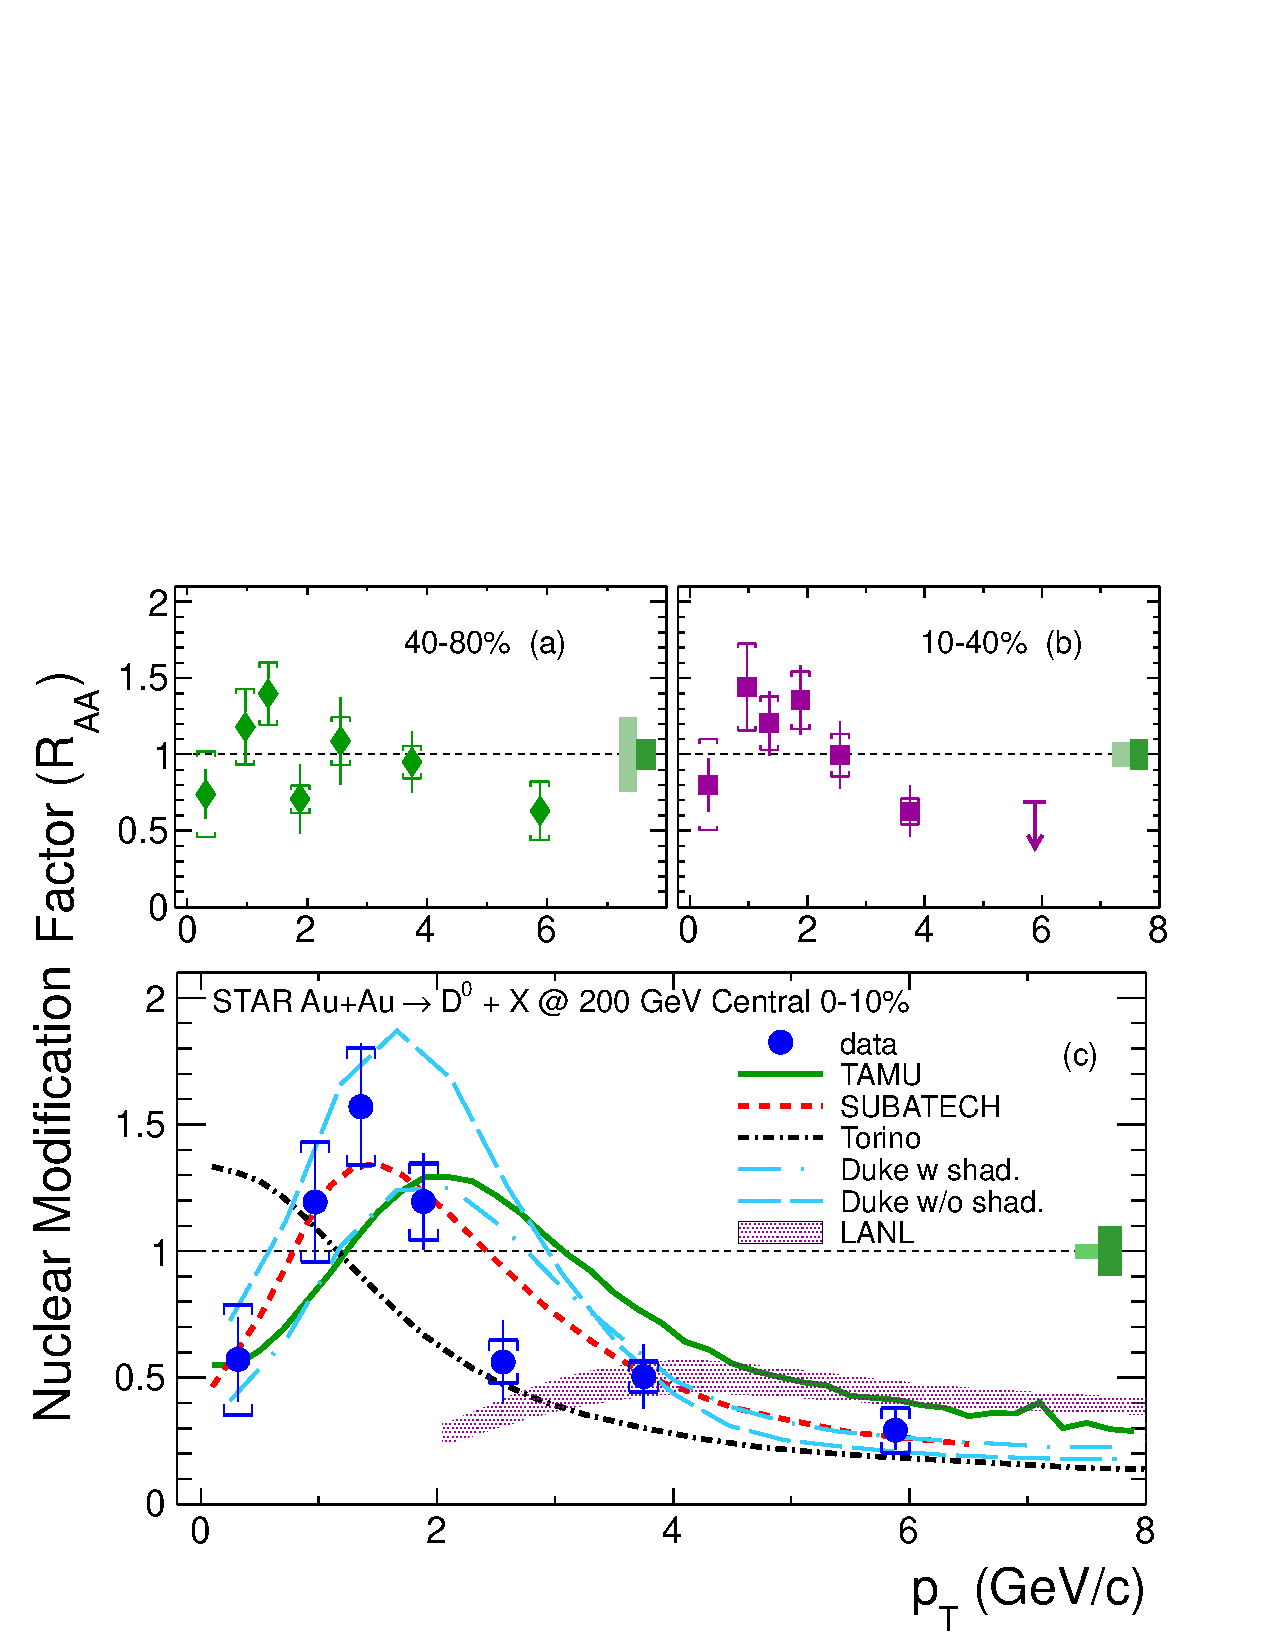
\includegraphics[width=0.90\textwidth]{fig/D-RAA-star} } 
 \caption[STAR measurements of $D$-meson production compared to theory]{Nuclear modification factor of $D$-mesons in 200 GeV \AuAu\ collisions 
 at various centralities as measured by STAR~\cite{Adamczyk:2014uip}, compared to 
 theoretical 
 calculations~\cite{Adil:2006ra,Gossiaux:2008jv,He:2011qa,Alberico:2013bza,Cao:2013ita} 
 } 
 \label{fig:D-RAA-star} 
 \end{figure} 
 Remarkable results for open heavy-flavor observables have recently been obtained at 
 both RHIC and the LHC. The STAR~\cite{Adamczyk:2014uip} and 
 ALICE~\cite{Alice:2012ab,Abelev:2013lca,Abelev:2014ipa} collaborations have, for the 
 first time, been able to extract the nuclear modification factor ($R_{AA}$) and 
 elliptic flow ($v_2$) of $D$ mesons. The STAR measurement of $D$ mesons in 200 GeV 
 Au-Au reaches down to rather low transverse momenta ($p_T$)~\cite{Adamczyk:2014uip}, 
 showing intriguing evidence for a maximum in the $R_{AA}(p_T)$ as seen in 
 Figure~\ref{fig:D-RAA-star}. Such a structure is a tell-tale signature for collective 
 behavior of $D$ mesons, which in turn requires a strong coupling of $c$ quarks and $D$ mesons 
 to the expanding medium. As part of the thermalization process, the heavy-flavor
 particles are dragged along in the fireball expansion and accumulate in a momentum range
 characteristic of the medium's collective flow velocity, while low- and high-momentum states are 
 depleted. This feature can be described by theoretical calculations which implement 
 (a) a sufficiently small diffusion coefficient of $ D_s (2\pi T) \leq5$ into dynamical 
 evolution models~\cite{He:2011qa,Gossiaux:2008jv,Cao:2013ita}, and 
 (b) heavy-light 
 quark coalescence in the hadronization process. The precise location of the
 flow bump turns out to be rather sensitive to the underlying bulk evolution model. 
 Systematic comparisons of the different ingredients to the theoretical models and 
 improved precision in the data are required to disentangle the different effects and 
 arrive at quantitative results for the heavy-quark transport coefficient. 
 Additionally, measurements of the $R_{AA}$ of $D_s$ mesons (containing one charm and 
 one strange anti-/quark), would be very helpful as coalescence processes of $c$ quarks 
 with the enhanced strangeness content of the QGP significantly augment the flow 
 bump~\cite{He:2012df}.  

 A critical role in the determination of the transport coefficient is played by measurements of the elliptic flow parameter
 $v_2$ of the heavy-flavor particles. Electrons and muons from semileptonic decays 
 of $D$- and $B$-meson have been found to carry a rather large $v_2$ in heavy ion
 collisions at both RHIC~\cite{Adare:2006nq,Mustafa:2012jh} and the LHC~\cite{Sakai:2013ata}. 
 Important midterm goals at RHIC are to disentangle the $B$ and $D$ contributions to the semileptonic decays, and to 
 obtain an independent measurement of the $v_2$ of directly reconstructed $D$ mesons. 
 The former will be extracted from existing RHIC 2014 Au+Au displaced vertex 
 measurements by PHENIX (using the VTX and FVTX detectors)~\cite{Nouicer:2012pr}, and by 
 STAR (using the HFT detector)~\cite{Kapitan:2008kk,Qiu:2014dha}. The $v_2$ of directly reconstructed $D$ mesons 
 will be obtained from the same data set using the STAR HFT~\cite{Qiu:2014dha}. 
 At the LHC, ALICE has 
 conducted first measurements of the $D$-meson $v_2$ in 2.76\,TeV \PbPb\ 
 collisions~\cite{Abelev:2013lca}, and found large values; CMS has been able to extract 
 a $B$-meson $R_{AA}$ through their displaced-vertex decays into $J/\psi$'s (so-called 
 non-prompt $J/\psi$'s~\cite{Chatrchyan:2012np}, which is approximately unity for small  
 momenta and turns into a suppression leveling off at $\sim$0.5 at high momenta. As 
 in the $D$-meson sector, this is consistent with collective behavior and thus indicative 
 for a strong bottom coupling to the medium, providing further valuable model constraints.

 An outstanding  issue is the determination of the temperature dependence of the transport coefficient.  
 Experimentally, one lever arm is provided by the correlation between $v_2$ and the 
 $R_{AA}$. Since the bulk medium $v_2$ takes several fm/$c$ to build up, a large $v_2$ 
 of the HF particles is indicative for a strong coupling in the later QGP phases of the 
 fireball evolution, and through hadronization. 
 A suppression in the $R_{AA}$, on the other hand, begins immediately in the early 
 high-density phases, especially at high $p_T$. Model calculations to date
 cannot easily account for the large $D$-meson $v_2$ at LHC without overestimating 
 the suppression in the $R_{AA}$. This corroborates a strong coupling in the vicinity
 of $T_{\rm c}$. The second lever arm is provided by going to lower collision 
 energies where the system starts out at smaller QGP temperatures, closer to $T_{\rm c}$. 
 First data for the heavy-flavor electron $R_{AA}$ and $v_2$ have been extracted
 from a 62\,GeV run at RHIC~\cite{Adare:2014rly,Adamczyk:2014yew}, and show evidence 
 for a non-vanishing $v_2$ and marked modifications in the $R_{AA}$. They are not 
 imcompatible with model calculations that utilize a strong heavy-flavor coupling around 
 $T_c$~\cite{He:2014epa}, but the data precision does not yet suffice for clear conclusions. 
 While varying the collision energy is a valuable tool to explore the temperature 
 dependence of these phenomena, it is necessary to account for the 
 more pronounced role of the Cronin effect at these energies, i.e., 
 a modification of the heavy-flavor spectra through cold nuclear matter effects, before 
 the QGP forms. 
Here  \pA\ collisions will be important to quantify these effects in order to provide a realistic starting 
point for assessing the hot-medium effects. 
 
  

%\bibliographystyle{atlasnote}
%\bibliography{OpenHeavyFlavor}

%\end{document}


